 %-------------------------------%
\begin{figure}[ht]\centering
    %-------------------------------%
    \newcommand{\scaleFactor}{0.7} % Define the scale factor
    \newcommand{\arrowN}[2]{\draw[arrow] (#1,#2+0.25-0.5) -- (#1,#2+0.75-0.5);} % North
    \newcommand{\arrowS}[2]{\draw[arrow] (#1,#2+0.75-0.5) -- (#1,#2+0.25-0.5);} % South
    \newcommand{\arrowE}[2]{\draw[arrow] (#1+0.25-0.5,#2) -- (#1+0.75-0.5,#2);} % East
    \newcommand{\arrowW}[2]{\draw[arrow] (#1+0.75-0.5,#2) -- (#1+0.25-0.5,#2);} % West
    \newcommand{\gridgreenredblack}{\foreach \x in {0,1,2,3}{\foreach \y in {0,1,2}	\node[box] at (\x,\y){};}
        \node[box, fill=green] at (3,2){{\boldmath $+1$}};
        \node[box, fill=red] at (3,1){{\boldmath $-1$}};
        \node[box, fill=black] at (1,1){};
    }
    \begin{subfigure}{.24\textwidth}
        \centering
        \scalebox{\scaleFactor}{%
            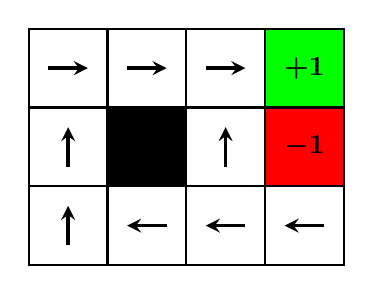
\begin{tikzpicture}
                [box/.style={rectangle,draw=black,thick, minimum size=1cm},
                arrow/.style={->,>=stealth,very thick},
                ]
                \gridgreenredblack
                \arrowE{0}{2}	\arrowE{1}{2}	\arrowE{2}{2}
                \arrowN{0}{1} 	\arrowN{2}{1}	
                \arrowN{0}{0}	\arrowW{1}{0}	\arrowW{2}{0}	\arrowW{3}{0}
            \end{tikzpicture}
        }
        \caption{$\varepsilon=-0.01$}
    \end{subfigure}
    \hfil
    \begin{subfigure}{0.24\textwidth}
        \centering
        \scalebox{\scaleFactor}{%
            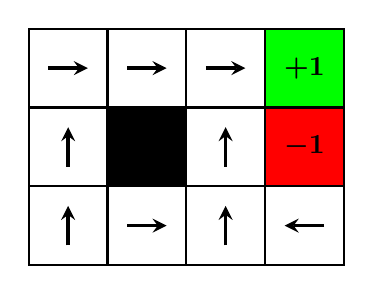
\begin{tikzpicture}
                [box/.style={rectangle,draw=black,thick, minimum size=1cm},
                arrow/.style={->,>=stealth,very thick},
                ]
                \gridgreenredblack
                \arrowE{0}{2}	\arrowE{1}{2}	\arrowE{2}{2}
                \arrowN{0}{1}	\arrowN{2}{1}
                \arrowN{0}{0} 	\arrowE{1}{0}	\arrowN{2}{0}	\arrowW{3}{0}
            \end{tikzpicture}
        }
        \caption{$\varepsilon=-0.1$}
    \end{subfigure}
    \hfil
    \begin{subfigure}{0.24\textwidth}
        \centering
        \scalebox{\scaleFactor}{%
            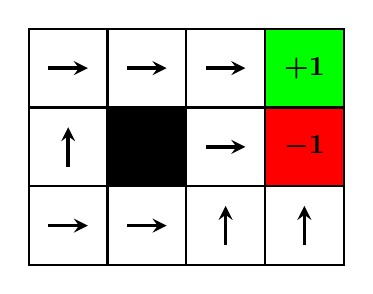
\begin{tikzpicture}
                [box/.style={rectangle,draw=black,thick, minimum size=1cm},
                arrow/.style={->,>=stealth,very thick},
                ]
                \gridgreenredblack
                \arrowE{0}{2}	\arrowE{1}{2}	\arrowE{2}{2}
                \arrowN{0}{1}	\arrowE{2}{1}
                \arrowE{0}{0}	\arrowE{1}{0}	\arrowN{2}{0}	\arrowN{3}{0}
            \end{tikzpicture}
        }
        \caption{$\varepsilon=-2$}
    \end{subfigure}
    \hfil
    \begin{subfigure}{0.25\textwidth}
        \centering
        \scalebox{\scaleFactor}{%
            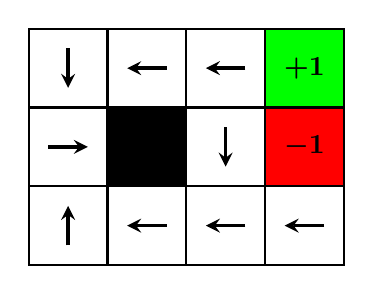
\begin{tikzpicture}
                [
                box/.style={rectangle,draw=black,thick, minimum size=1cm},
                arrow/.style={->,>=stealth,very thick},
                ]
                \gridgreenredblack
                \arrowS{0}{2}	\arrowW{1}{2}	\arrowW{2}{2}
                \arrowE{0}{1}	\arrowS{2}{1}
                \arrowN{0}{0}	\arrowW{1}{0}	\arrowW{2}{0}	\arrowW{3}{0}
            \end{tikzpicture}
        }
        \caption{$\varepsilon=0.01$}
    \end{subfigure}
    % \caption{Optimal policies for the slippery gridworld environment for various choices of
    %     penalty $\varepsilon$.}
\end{figure}